\documentclass[a4paper,12pt]{report}
% Alternative Options:
%	Paper Size: a4paper / a5paper / b5paper / letterpaper / legalpaper / executivepaper
% Duplex: oneside / twoside
% Base Font Size: 10pt / 11pt / 12pt

\usepackage[export]{adjustbox}

\usepackage{geometry}
%% Language %%%%%%%%%%%%%%%%%%%%%%%%%%%%%%%%%%%%%%%%%%%%%%%%%
%\usepackage[USenglish]{babel} %francais, polish, spanish, ...
\usepackage[francais]{babel}
\usepackage[T1]{fontenc}
\usepackage[latin1]{inputenc}

\usepackage{verbatim}
\usepackage{lmodern} %Type1-font for non-english texts and characters


%% Packages for Graphics & Figures %%%%%%%%%%%%%%%%%%%%%%%%%%
\usepackage{graphicx} %%For loading graphic files
%\usepackage{subfig} %%Subfigures inside a figure
%\usepackage{pst-all} %%PSTricks - not useable with pdfLaTeX

%% Please note:
%% Images can be included using \includegraphics{Dateiname}
%% resp. using the dialog in the Insert menu.
%% 
%% The mode "LaTeX => PDF" allows the following formats:
%%   .jpg  .png  .pdf  .mps
%% 
%% The modes "LaTeX => DVI", "LaTeX => PS" und "LaTeX => PS => PDF"
%% allow the following formats:
%%   .eps  .ps  .bmp  .pict  .pntg


%% Math Packages %%%%%%%%%%%%%%%%%%%%%%%%%%%%%%%%%%%%%%%%%%%%
\usepackage{amsmath}
\usepackage{amsthm}
\usepackage{amsfonts}


%% Line Spacing %%%%%%%%%%%%%%%%%%%%%%%%%%%%%%%%%%%%%%%%%%%%%
\usepackage{setspace}
%\singlespacing        %% 1-spacing (default)
%\onehalfspacing       %% 1,5-spacing
%\doublespacing        %% 2-spacing
\usepackage{listings}
\lstset{language=C++} 
\usepackage{color}

\definecolor{mygreen}{rgb}{0,0.6,0}
\definecolor{mygray}{rgb}{0.5,0.5,0.5}
\definecolor{mymauve}{rgb}{0.58,0,0.82}

\lstset{ %
  backgroundcolor=\color{white},   % choose the background color; you must add \usepackage{color} or \usepackage{xcolor}
  basicstyle=\footnotesize,        % the size of the fonts that are used for the code
  breakatwhitespace=false,         % sets if automatic breaks should only happen at whitespace
  breaklines=true,                 % sets automatic line breaking
  captionpos=b,                    % sets the caption-position to bottom
  commentstyle=\color{mygreen},    % comment style
  deletekeywords={...},            % if you want to delete keywords from the given language
  escapeinside={\%*}{*)},          % if you want to add LaTeX within your code
  extendedchars=true,              % lets you use non-ASCII characters; for 8-bits encodings only, does not work with UTF-8
  frame=single,                    % adds a frame around the code
  keepspaces=true,                 % keeps spaces in text, useful for keeping indentation of code (possibly needs columns=flexible)
  keywordstyle=\color{blue},       % keyword style
  language=C++,                 % the language of the code
  otherkeywords={*,...},            % if you want to add more keywords to the set
  numbers=left,                    % where to put the line-numbers; possible values are (none, left, right)
  numbersep=5pt,                   % how far the line-numbers are from the code
  numberstyle=\tiny\color{mygray}, % the style that is used for the line-numbers
  rulecolor=\color{black},         % if not set, the frame-color may be changed on line-breaks within not-black text (e.g. comments (green here))
  showspaces=false,                % show spaces everywhere adding particular underscores; it overrides 'showstringspaces'
  showstringspaces=false,          % underline spaces within strings only
  showtabs=false,                  % show tabs within strings adding particular underscores
  stepnumber=2,                    % the step between two line-numbers. If it's 1, each line will be numbered
  stringstyle=\color{mymauve},     % string literal style
  tabsize=2,                       % sets default tabsize to 2 spaces
  title=\lstname                   % show the filename of files included with \lstinputlisting; also try caption instead of title
}







%% NOTE POUR CLEMENT : UTILISE LE HEADER CI-DESSUS, IL EST MEILLEUR

%%AJOUTS DE CLEMENT DANS LE HEADER :
\usepackage{fancyhdr}
\pagestyle{fancy}
\lhead{Clément BLANQUET et Rafik CHENNOUF}
\rhead{Page \thepage}
\cfoot{\footnotesize{MI11 - Rapport des TPs : Réalisation d'un mini noyau temps réel}}
\renewcommand{\headrulewidth}{0.4pt}
\renewcommand{\footrulewidth}{0.4pt}

\usepackage{titlesec}
\makeatletter
\titleformat{\chapter}[frame]
  {\normalfont}{\filright\enspace \@chapapp~\thechapter\enspace}
  {15pt}{\LARGE\bfseries\filcenter}
\titlespacing*{\chapter}
  {0pt}{0pt}{20pt}
\makeatother

\renewcommand{\thesection}{}
\renewcommand{\thesubsection}{\arabic{section}.\arabic{subsection}}
\makeatletter
\def\@seccntformat#1{\csname #1ignore\expandafter\endcsname\csname the#1\endcsname\quad}
\let\sectionignore\@gobbletwo
\let\latex@numberline\numberline
\def\numberline#1{\if\relax#1\relax\else\latex@numberline{#1}\fi}
\makeatother

\usepackage{animate}
\usepackage{hyperref}




\author{Clément BLANQUET et Rafik CHENNOUF}
\title{MI11 - Rapport des TPs : Réalisation d'un mini noyau temps réel}

\begin{document}

\begin{titlepage}

	\centering
	
\includegraphics[width=0.15\textwidth]{sigle_UTC.jpg}\par\vspace{1cm}
	{\scshape\LARGE Université de Technologie de Compiègne \par\vspace{1cm}}	
	{\scshape\Large MI11\par}
	\vspace{1.5cm}
	{\huge\bfseries Rapport des TPs : Réalisation d'un mini noyau temps réel\par}
	\vspace{2cm}
	{\Large\itshape Clément BLANQUET et Rafik CHENNOUF\par}
	\vspace{2cm}
	\vfill
% Bottom of the page
	{\large Juin 2017}
\end{titlepage}


\renewcommand{\contentsname}{Sommaire} % Changer le nom de la table des matieres
\tableofcontents
% Les différentes tables
\listoffigures        % Liste des figures




\chapter{Rapport TP 1 - Partie 1 et 2}

\section{1ère partie : Ordonnanceur de tâches}

Voici comment nous avons codé les fonctions \textit{file\_init()}, \textit{ajoute(n)}, \textit{suivant()} et \textit{retire(n)} :

\subsection{file\_init()}
Cette fonction permet simplement d'initialiser la file FIFO de tâches.
\begin{lstlisting}
void	file_init( void )
{
	int i;
	_queue=F_VIDE;

	for (i=0;i<MAX_TACHES;i++)
		_file[i]=F_VIDE;
}
\end{lstlisting}

Dans cette fonction, on se contente d'initialiser la queue da la file FIFO à la valeur F\_VIDE (F\_VIDE = MAX\_TACHES = 8), ce qui signifie que la file est vide. De plus, on initialise chaque case du tableau représentant la file à la même valeur, indiquant que chaque case est vide.


\subsection{ajoute(n)}
Cette fonction permet d'ajouter une tâche en fin de file.
\begin{lstlisting}
void	ajoute ( uint16_t n )
{
	if(n > MAX_TACHES - 1) // Si le numéro de la tâche est trop grand
		return;

	if(_queue == F_VIDE) // Si la file est vide
	{
		_queue = n;
		_file[_queue] = n;
	}
	else // La file n'est pas vide
	{
		uint16_t tmp = _file[_queue];
		_file[_queue] = n;
		_file[n] = tmp;
		_queue = n;
	}
}
\end{lstlisting}

La fonction \textit{ajoute} prend en argument un entier qui représente le numéro de la tâche à ajouter.\smallbreak

On commence par regarder si le numéro de la tâche à ajouter est cohérent (inférieur ou égal à 7). Si ce n'est pas le cas, on sort de la fonction.\smallbreak

Sinon, si la file est vide (\_queue = F\_vide), la queue devient la tâche qui vient d'être ajoutée et le successeur de cette tâche est elle-même.\smallbreak

Enfin, si la file n'est pas vide, on veut ajouter la nouvelle tâche en fin de file. Autrement dit, la queue doit valeur cette même nouvelle tâche. On commence par sauvegarder dans un tampon le successeur de la queue actuelle. Ensuite, on désigne la nouvelle tâche comme étant le successeur de la queue actuelle. De plus, on désigne le successeur de la nouvelle tâche comme étant la tâche sauvegardée dans le tampon, anciennement successeur de la queue actuelle. Enfin, on désigne notre nouvelle tâche comme étant la queue.\smallbreak

De cette façon, la nouvelle tâche s'est intercalée entre l'ancienne queue et son ancien successeur, et est devenue la nouvelle queue.


\subsection{suivant()}
Cette fonction retourne la tâche à activer, et met à jour \_queue pour qu'elle pointe sur la suivante.
\begin{lstlisting}
uint16_t	suivant( void )
{
	_queue = _file[_queue];
	return _queue;
}
\end{lstlisting}

Ici on assigne à la queue son successeur (donc la tâche à activer) puis on la retourne.


\subsection{retire(n)}
Cette fonction permet de retirer une tâche de la file sans en modifier l'ordre.
\begin{lstlisting}
void	retire( uint16_t t )
{
	int i = 0;

	if(t > MAX_TACHES || _queue == F_VIDE)
		return;

	while(_file[i] != t)
		i++;				// i = prédecesseur de t 
							  // ex : ( 1 -> 0 -> 2 ) => avec t = 0, i = 1

	if(i == MAX_TACHES)
		return;

	_file[i] = _file[t];	// 1 -> 2
	_file[t] = F_VIDE;
	
	if(t == _queue)
	{
		// si le prédécesseur est lui même => une seule tâche => queue => on vide
		if(t == i)			
			_queue = F_VIDE;
		else
			_queue = i;		// la queue devient le prédécesseur de la tâche qu'on retire
	}
}
\end{lstlisting}

La fonction prend en argument le numéro de la tâche à retirer. On commence donc par vérifier que ce numéro est cohérent (inférieur ou égal à 7) et que la file n'est pas vide auquel cas il est impossible de retirer un élément.\smallbreak

Une fois cette vérification effectuée, on cherche le prédecesseur de la tâche à retirer. Si on ne trouve rien, cela signifie que la tâche n'existe pas et on sort donc de la fonction.\smallbreak

Sinon, on "saute au dessus" de la tâche à retirer, c'est à dire qu'on fixe le successeur du prédécesseur de cette tâche comme étant le successeur de cette même tâche.\smallbreak

Enfin, on doit vérifier si la tâche retirée était la queue ou non.
\begin{itemize}
\item Si oui
	\begin{itemize}
	\item Si la file ne contient qu'un élément (donc le prédécesseur de la tâche est la tâche elle-même), on assigne à \_queue la valeur F\_VIDE (car la file est alors vide)
	\item Sinon, la queue devient le prédécesseur de la tâche que l'on a retiré.
	\end{itemize}
\item Sinon, ne rien faire de plus.
\end{itemize}


\subsection{affic\_file()}
Cette fonction permet d'afficher la file.
\begin{lstlisting}
void affic_file( void )
{
	int i = 0;

	// Recherche du premier élément de la file
	while (_file[i] == F_VIDE) 
		i++;

	int temp = i; // temp ==> premier élément de la file

	// Tant qu'on a pas fait tout le tour de la file
	while (_file[i] !=temp) 
	{
		// Si l'élément i est la queue, afficher un "(Q)" à côté
		if (i==_queue)
			printf(" %d(Q) -> ", i); 
		else
				printf(" %d -> ", i); // Sinon l'afficher normalement
				
		i=_file[i]; // Passer à l'élément suivant
	}
	// Affichage du dernier élément
	if (i==_queue)
		printf(" %d (Q) -> ", i);
	else
		printf(" %d -> ", i);

	printf("\n");
}
\end{lstlisting}

On commence par chercher le premier élément de la file. Ensuite, on effectue une boucle d'affichage tant qu'un tour complet de la file n'a pas été effectué. On affiche "(Q)" à côté de la tâche sur laquelle la queue pointe.



\subsection{Test de ces fonctions}
Nous avons pu tester le bon fonctionnement de ces fonctions grâce au fichier de test \textit{testfile.c} suivant :
\begin{lstlisting}
#include "noyau.h"
#include "serialio.h"


int main()
{
	serial_init(115200);
	
	printf("***********************************\n");

	file_init();

	// Ajouts des différentes tâches comme dans l'exemple du sujet
	ajoute(3);
	ajoute(5);
	ajoute(1);
	ajoute(0);
	ajoute(2);

	affic_file(); // Affichage de la file

	affic_queue(); // Affichage de la queue
	printf("Suivant() \n");
	suivant(); // On fait un "suivant()"
	affic_queue(); // On vérifie la queue après le "suivant()"

	affic_file(); // Affichage de la file avec la nouvelle queue

	printf("Retire 0 : \n");
	retire(0); // On retire la tâche 0
	affic_file(); // Affichage de la file après le "retire(0)"
	printf("Ajoute 6 : \n");
	ajoute(6); // On ajoute 6
	affic_file(); // Affichage de la file après le "ajoute(6)"

	return 0;
}
\end{lstlisting}
\newpage
A l'exécution, on obtient :
\begin{figure}[h]
	\centering
		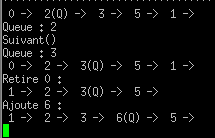
\includegraphics[width=0.5\textwidth]{screens/tp1/Exo1_NEW.PNG}
		\caption{Résultat de testfile.c}
		\label{testfile}
\end{figure}

C'est bien le résultat attendu. En effet, au départ la queue vaut 2 car c'est la dernière tâche à avoir été ajoutée. Après le suivant, la valeur de la queue change et devient le successeur de 2 à savoir 3, ce qui s'affiche correctement. Le \textit{retire(0)} fonctionne bien aussi puisque la tâche 0 a disparu de la file et les autres tâches ont leurs successeurs et prédécesseurs bien mis à jour. Enfin, le ajoute(6) ajoute bien la tâche 6 en fin de file en mettant à jour la queue.

\newpage
\section{2ème partie : gestion et commutation de tâches}
Dans cette seconde partie, nous devons réaliser  les  primitives de  gestion  des  tâches  du  mini  noyau  temps réel, ainsi que le système de commutation de tâches. Tout cela est écrit dans le fichier \textit{noyau.c}.

Les codes nous étant fournis, nous devons les expliquer. Notons tout d'abord les variables internes au noyau :

\begin{lstlisting}
static int compteurs[MAX_TACHES]; // Compteurs d'activations 
CONTEXTE _contexte[MAX_TACHES];   // tableau des contextes 
volatile uint16_t _tache_c;       // numéro de tache courante 
uint32_t  _tos;                   // adresse du sommet de pile 
int  _ack_timer = 1;          // = 1 si il faut acquitter le timer 
\end{lstlisting}



\subsection{Fonction noyau\_exit()}
\begin{lstlisting}
void	noyau_exit(void)
{
  int j;
  _irq_disable_();                // Désactiver les interruptions 
  printf("Sortie du noyau\n");
  for (j=0; j < MAX_TACHES; j++)
    printf("\nActivations tache %d : %d", j, compteurs[j]);
  for(;;);                        // Terminer l'exécution 
}
\end{lstlisting}

Commençons par la fonction \textit{noyau\_exit()} qui permet de sortir du noyau (donc d'arrêter tout).
Les interruptions sont désactivées et juste avant de sortir du noyau (en faisant une boucle infinie), on affiche le nombre de fois que chaque tâche a été activée grâce au tableau \textit{compteurs}.

\subsection{Fonction fin\_tache()}
\begin{lstlisting}
void  fin_tache(void)
{
  // on interdit les interruptions
  _irq_disable_();
  // la tache est enlevee de la file des taches
  _contexte[_tache_c].status = CREE;
  retire(_tache_c);
  schedule();
}
\end{lstlisting}

Cette fonction permet de rendre une tâche inactive alors qu'elle était active jusqu'alors. Pour cela, après avoir interdit les interruptions, on change son statut à "CREE" ce qui fait que la tâche n'est plus prête à être exécutée. Elle reste tout de même connue du noyau et est simplement en attente. On la retire de la FIFO grâce à notre fonction \textit{retire()} créée dans la première partie. A la fin, on lance la fonction \textit{schedule()} (que l'on étudiera par la suite) pour que les tâches suivantes puissent s'exécuter. En fait, on appelle cette fonction à la fin de chaque tâche pour y mettre fin.

\subsection{Fonction cree(TACHE\_ADR adr\_tache)}
\begin{lstlisting}
uint16_t cree( TACHE_ADR adr_tache )
{
  CONTEXTE *p;                    // pointeur d'une case de _contexte 
  static   uint16_t tache = -1;   // contient numero dernier cree 


  _lock_();                       // debut section critique 
  tache++;                        // numero de tache suivant 

  if (tache >= MAX_TACHES)        // sortie si depassement 
    noyau_exit();

  p = &_contexte[tache];          // contexte de la nouvelle tache 

  p->sp_ini = _tos;               // allocation d'une pile a la tache 
  _tos -= PILE_TACHE + PILE_IRQ;  // decrementation du pointeur de pile pour la prochaine tache

  _unlock_();                     // fin section critique 

  p->tache_adr = adr_tache;       // memorisation adresse debut de tache 
  p->status = CREE; 		          // mise a l'etat CREE 
  return(tache);                  // tache est un uint16_t 
}
\end{lstlisting}

La fonction \textit{cree} permet de créer une tâche et de lui allouer une pile et un numéro. On commence tout d'abord par incrémenter le nombre de tâches créées via la variable \textit{tache}. On récupère ensuite le contexte de la nouvelle tâche via le pointeur \textit{p}. Le pointeur de pile associé à la tâche pointe à l'adresse du sommet de pile (\textit{\_tos}) ce qui permet d'allouer une pile à la tâche. On décrémente ensuite le pointeur de pile par la taille maximale de la pile d'une tâche + la taille maximale de la pile IRQ par tâche. Ceci permet d'allouer assez de place pour la tâche suivante. Enfin, on enregistre l'adresse de début de la tâche et on passe le statut de la tâche à "CREE".	


\subsection{Fonction active( uint16\_t tache )}
\begin{lstlisting}
void  active( uint16_t tache )
{
  CONTEXTE *p = &_contexte[tache]; // acces au contexte tache

  if (p->status == NCREE)
    noyau_exit();                 // sortie du noyau 

  _lock_();                       // debut section critique 
  if (p->status == CREE)          // n'active que si receptif 
  {
    p->status = PRET;             // changement d'etat, mise a l'etat PRET 
    ajoute(tache);                // ajouter la tache dans la liste 
    schedule();                		// activation d'une tache prete 
  }
  _unlock_();                     // fin section critique 
}
\end{lstlisting}
Cette fonction place une tâche dans la file d'attente des tâches éligibles.  Elle prend en entrée le numéro de la tâche.

On vérifie d'abord si la tâche est bien créée. Si c'est le cas, alors on va modifier le statut de la tâche (de CREE à PRET) et l'ajouter à notre FIFO (on rentre donc dans une section critique). On finit par lancer un \textit{schedule()} pour activer la prochaine tâche.


\subsection{Fonction scheduler}
\begin{lstlisting}
void __attribute__((naked)) scheduler( void )
{
  register CONTEXTE *p;
  register unsigned int sp asm("sp");  // Pointeur de pile  

  // Sauvegarder le contexte complet sur la pile IRQ  
  __asm__ __volatile__(
      "stmfd  sp, {r0-r14}^\t\n"  // Sauvegarde registres mode system  
      "nop\t\n"                   // Attendre un cycle  
      "sub    sp, sp, #60\t\n"    // Ajustement pointeur de pile  
      "mrs    r0, spsr\t\n"       // Sauvegarde de spsr_irq  
      "stmfd  sp!, {r0, lr}\t\n");// et de lr_irq  

  if (_ack_timer)                 // Réinitialiser le timer si nécessaire  
  {
    register struct imx_timer* tim1 = (struct imx_timer *) TIMER1_BASE;
    tim1->tstat &=~TSTAT_COMP;
  }
  else
  {
    _ack_timer = 1;
  }

  _contexte[_tache_c].sp_irq = sp;// memoriser le pointeur de pile  
  _tache_c = suivant();           // recherche du suivant  
  if (_tache_c == F_VIDE)
  {
    printf("Plus rien à ordonnancer.\n");
    noyau_exit();                 // Sortie du noyau  
  }
  compteurs[_tache_c]++;          // Incrémenter le compteur d'activations   
  p = &_contexte[_tache_c];       // p pointe sur la nouvelle tache courante 

  if (p->status == PRET)          // tache prete ?  
  {
    sp = p->sp_ini;               // Charger sp_irq initial  
    _set_arm_mode_(ARMMODE_SYS);  // Passer en mode système  
    sp = p->sp_ini - PILE_IRQ;    // Charger sp_sys initial  
    p->status = EXEC;             // status tache -> execution  
    _irq_enable_();               // autoriser les interuptions    
    (*p->tache_adr)();            // lancement de la tâche  
  }
  else
  {
    sp = p->sp_irq;               // tache deja en execution, restaurer sp_irq  
  }

  // Restaurer le contexte complet depuis la pile IRQ  
  __asm__ __volatile__(
      "ldmfd  sp!, {r0, lr}\t\n"  // Restaurer lr_irq  
      "msr    spsr, r0\t\n"       // et spsr_irq  
      "ldmfd  sp, {r0-r14}^\t\n"  // Restaurer registres mode system  
      "nop\t\n"                   // Attendre un cycle  
      "add    sp, sp, #60\t\n"    // Ajuster pointeur de pile irq  
      "subs   pc, lr, #4\t\n");   // Retour d'exception  
}
\end{lstlisting}

Cette fonction fait office d'ordonnanceur de tâches. On rappelle que cette fonction s'exécute en mode IRQ. On commence tout d'abord par sauvegarder le contexte complet sur la pile IRQ car nous allons modifié le pointeur de pile \textit{sp} du mode IRQ dans la fonction. On exécute ensuite la fonction \textit{suivant()} pour récupérer la tâche à activer. Si cette tâche est vide alors il n'y a plus rien à ordonnancer donc on quitte le noyau. Sinon, on incrémente le compteur d'activations associé à cette tâche pour spécifier que cette tâche a été activée une fois de plus. Pour activer la tâche, il faut qu'elle soit en mode "PRET" sinon cela veut dire que la tâche est déjà en exécution. Dans ce deuxième cas, on met juste à jour le pointeur de pile \textit{sp} du mode IRQ avec la valeur courante du pointeur de pile associé à la tâche. Dans le premier cas, si la tâche est en mode "PRET" alors il faut que le pointeur de pile \textit{sp} en mode SYSTEM pointe sur la pile associé à la tâche. Pour cela, on passe en mode SYSTEM puis on affecte au pointeur de pile \textit{sp} du mode SYSTEM la valeur initiale du pointeur de pile associé à la tâche - la taille maximale de la pile IRQ par tâche. On passe ensuite le statut de la tâche en "EXEC" pour qu'elle soit exécutable puis on exécute la tâche. Enfin, on restaure le contexte complet depuis la pile IRQ.



\subsection{Fonction schedule()}
\begin{lstlisting}
void  schedule( void )
{
  _lock_();                         // Debut section critique  

  // On simule une exception irq pour forcer un appel correct à scheduler(). 
  _ack_timer = 0;
  _set_arm_mode_(ARMMODE_IRQ);      // Passer en mode IRQ  
  __asm__ __volatile__(
      "mrs  r0, cpsr\t\n"           // Sauvegarder cpsr dans spsr  
      "msr  spsr, r0\t\n"
      "add  lr, pc, #4\t\n"         // Sauvegarder pc dans lr et 																		// l'ajuster  
      "b    scheduler\t\n"          // Saut à scheduler  
      );
  _set_arm_mode_(ARMMODE_SYS);      // Repasser en mode system  

  _unlock_();                       // Fin section critique  
}
\end{lstlisting}
La fonction \textit{schedule()} permet en fait de faire un appel à la fonction \textit{scheduler()}. Dans une section critique, elle commence par passer en mode IRQ (car la fonction \textit{scheduler} doit s'exécuter dans ce mode). Ensuite, en assembleur, on sauvegarde le registre \textbf{CPSR} dans \textbf{SPSR}. On rappelle que le registre \textbf{SPSR} est disponible dans chaque mode d'exception dont IRQ. Il est destiné à recevoir la sauvegarde du registre \textbf{CPSR} du programme interrompu. On poursuit en sauvegardant \textbf{pc} dans \textbf{lr} et on l'ajuste car après l'exécution de \textit{scheduler} il faut revenir à ce niveau. On lance ensuite \textit{scheduler} et on repasse en mode SYSTEM.


\subsection{Fonction start( TACHE\_ADR adr\_tache )}
\begin{lstlisting}
void	start( TACHE_ADR adr_tache )
{
  short j;
  register unsigned int sp asm("sp");
  struct imx_timer* tim1 = (struct imx_timer *) TIMER1_BASE;
  struct imx_aitc* aitc = (struct imx_aitc *) AITC_BASE;

  for (j=0; j<MAX_TACHES; j++)
  {
    _contexte[j].status = NCREE;    // initialisation de l'etat des taches 
  }
  _tache_c = 0;                     // initialisation de la tache courante 
  file_init();                      // initialisation de la file           

  _tos = sp;                        // Haut de la pile des tâches 
  _set_arm_mode_(ARMMODE_IRQ);      // Passer en mode IRQ 
  sp = _tos;                        // sp_irq initial 
  _set_arm_mode_(ARMMODE_SYS);      // Repasser en mode SYS 

  _irq_disable_();                  // on interdit les interruptions 

  // Initialisation du timer à 100 Hz 
  tim1->tcmp = 10000;
  tim1->tprer = 0;
  tim1->tctl |= TCTL_TEN | TCTL_IRQEN | TCTL_CLKSOURCE_PERCLK16;

  // Initialisation de l'AITC 
  aitc->intennum = TIMER1_INT;

  active(cree(adr_tache));          // creation et activation premiere tache 
}
\end{lstlisting}

Cette fonction permet de lancer la première tâche et donc de lancer le système.
On commence par initialiser les statuts des tâches à "NCREE", la FIFO et la tâche courante à 0. L'adresse du sommet de la pile (\textit{\_tos}) est ensuite mis à jour avec la valeur du pointeur de pile \textit{sp} en mode SYSTEM car on s'apprête à lancer la première tâche. On passe ensuite en mode IRQ pour mettre à jour le pointeur de pile \textit{sp} du mode IRQ qui lui pointe vers l'adresse du sommet de la pile. On repasse en mode SYSTEM puis on crée et on active la tâche pour lancer le système.









\chapter{Rapport TP 2 - Partie 3 et 4}

Le but de ce TP est d'implémenter des fonctions d'exclusions mutuelles afin que plusieurs tâches ne puissent pas accéder à une section critique en même temps au risque de créer un interblocage.  


\section{Exercice 1 : Exclusion mutuelle}

Tout d'abord, il est possible de faire du partage de ressources en agissant directement sur les tâches dépendantes en les faisant s'endormir ou se réveiller selon la situation. Dès qu'une tâche a terminée son accès à la mémoire partagée elle s'endort et réveille l'autre tâche afin qu'elle puisse y avoir accès et vis-versa.

\subsection{Suspension d'une tâche}

L'endormissement d'une tâche se fait via la primitive \textit{dort()} du fichier \textbf{noyau.c}.
Le but de cette fonction est de suspendre la tâche courante qui passe donc de l'état \textbf{EXEC} pour 'exécuter' à l'état \textbf{SUSP} pour 'suspendre'. La tâche est ensuite retirée de la file des tâches et un appel à l'ordonnanceur est réalisé afin de charger la tâche suivante. De plus, toutes ces opérations constituent une section critique qui ne doivent pas être exécutées en même temps par plusieurs fonctions. C'est pour cela qu'il faut les protéger avec un \textit{mutex} ou un \textit{lock}.\newline

Ci-dessous le code de la fonction \textit{dort()} :

\begin{lstlisting}
void  dort(void)
{
	_lock_();				// section critique

	CONTEXTE *p = &_contexte[_tache_c];
	p->status = SUSP;	// suspension

	retire(_tache_c);	// retirer la tâche
	schedule();

	_unlock_();
}
\end{lstlisting}

\subsection{Réveil d'une tâche}

Le réveil d'une tâche se fait via la primitive \textit{reveille()} du fichier \textbf{noyau.c}.
Cette primitive fonctionne de la même manière que la fonction \textit{dort()} vue précédemment sauf que l'état de la tâche courante est passé en mode EXEC au lieu de SUSP afin que la tâche puisse être exécutable par l'ordonnanceur après l'avoir ajoutée dans la file.\newline

Ci-dessous le code de la fonction \textit{reveille()} :

\begin{lstlisting}
void reveille(uint16_t t)
{

	// on vérifie que la tâche existe et est suspendue
	if(t > MAX_TACHES || _contexte[t].status != SUSP)	 
		return;

	_lock_();		// section critique

	CONTEXTE *p = &_contexte[t];
	p->status = EXEC;		// exécution

	ajoute(t);		// ajout dans la file
	schedule();

	_unlock_();
}
\end{lstlisting}

\subsection{Modèle de communications producteur/consommateur.}

Afin de tester nos deux primitives \textit{dort()} et \textit{reveille()}, nous avons implémenté le modèle de communications producteur/consommateur. Tout d'abord le programme comporte deux tâches; la première, le producteur, produit des entiers dans une file circulaire, la seconde, le consommateur, retire ces entiers de la file et les affiche.\newline

Pour faire cela, nous disposons d'une FIFO sous forme d'un tableau d'entiers de taille fixée (3 dans notre cas). On distingue 4 cas possibles :

1) Le producteur a tellement produit que la file est pleine => il s'endort.\newline
2) Le producteur a produit au moins un entier, la file est non vide => il réveille le consommateur pour qu'il consomme un ou des entiers.\newline
3) La file est vide car le producteur n'y a rien produit => le consommateur s'endort.\newline
4) Il reste encore de la place dans la file, la file est non pleine => le producteur se réveille pour produire des entiers.\newline

Pour gérer tous ces cas, nous possédons une variable qui compte le nombre de places libres et qui est, au début du programme, initialisée à la taille du tableau. Lorsque le nombre de places libres est supérieur ou égal à 1, le producteur produit un entier dans la file puis décrémente le nombre de places libres. De même, si le nombre de places libres est inférieur à la taille totale de la file alors le consommateur consomme un entier puis incrémente le nombre de places libres.\newline
Le cas 1 se produit lorsque la file est pleine, c'est à dire lorsque le nombre de places libres est égal à 0. 
Le cas 2 se produit lorsque la file est non vide,  c'est à dire lorsque le nombre de places libres est inférieur à la taille totale de la file.
Le cas 3 se produit lorsque la file est vide,  c'est à dire lorsque le nombre de places libres est égal à la taille totale de la file.
Le cas 4 se produit lorsque la file est non pleine, c'est à dire lorsque le nombre de places libres est égal à 1.\newline

En résumé, le producteur produit des entiers dans la file tant que celle-ci n'est pas pleine sinon il s'endort et le consommateur lit ces entiers tant que la file n'est pas vide sinon il s'endort. Lorsqu'il y a la moindre place dans la file, le consommateur réveille le producteur et lorsqu'il y a le moindre entier dans la file, le producteur réveille le consommateur.
A noté aussi que l'accès à la file représente une zone critique qu'il faut protéger via un \textit{lock}.
Initialement, seul le producteur est réveillé et le consommateur est endormi car il faut pouvoir produire au moins un entier.\newline

Nous avons testé deux cas de figures, un cas où le producteur est plus rapide que le consommateur et le cas inverse.\newline

Ci-dessous le code du modèle de communications producteur/consommateur dans le cas où le consommateur est plus rapide que le producteur :

\begin{lstlisting}
#define TAILLE_TABLEAU 3	

TACHE tacheStart();
TACHE tacheProd();
TACHE tacheConso();
uint16_t prod, conso;
uint16_t fifo[TAILLE_TABLEAU];	// la file
uint16_t nb_places_libres = TAILLE_TABLEAU;

TACHE	tacheStart(void)		// tâche de démarrage
{
  puts("------> EXEC tache Start");
  prod = cree(tacheProd);
  conso = cree(tacheConso);

  active(prod);
  active(conso);

  fin_tache();
}

TACHE	tacheProd(void)		// tâche producteur
{
  puts("------> EXEC tache Prod");

  uint16_t j=0,k,i=0;

  while(1)
  {
	  for (k=0; k<30000; k++);		// producteur plus lent

	  if (nb_places_libres>=1)		// production d'un entier
	  {
		  _lock_();									// zone critique
		  printf("**PROD** -> Production : fifo[%d] = %d\n", i, j);
		  fifo[i]=j;
		  _unlock_();
		  j++;

		  nb_places_libres--;

		  i++;
		  if (i==TAILLE_TABLEAU)	// i = indice de la file
			  i=0;
	  }
	  else			// file pleine
	  {
		  _lock_();
		  puts("**PROD** -> Producteur dort (Cas 1 : File pleine)\n");
		  _unlock_();

		  dort();		// producteur s'endort
	  }

	  if (nb_places_libres<TAILLE_TABLEAU)	// file non vide
	  {
		  _lock_();
		  puts("**PROD** -> Reveil du conso (Cas 2 : File non vide)\n");
		  _unlock_();

		  reveille(conso);		// consommateur se réveille
	  }

  }

  fin_tache();
}

TACHE	tacheConso(void)		// tâche consommateur
{
  uint16_t k,i=0;

  puts("------> EXEC tache Conso");

  dort();		// consommateur dort initialement

  while(1)
  {
	  for (k=0; k<10000; k++);	// consommateur plus rapide

	  if (nb_places_libres==TAILLE_TABLEAU)	// file vide
	  {
		  _lock_();
		  puts("**CONSO** -> Consommateur dort (Cas 3 : File vide)\n");
		  _unlock_();

		  dort();		// consommateur s'endort
	  }
	  else
	  {
		  _lock_();
		  printf("**CONSO** -> Lecture de fifo[%d] = %d\n", i, fifo[i]);
		  _unlock_();

		  nb_places_libres++;

		  i++;
		  if (i==TAILLE_TABLEAU)	// i = indice de la file
			  i=0;
	  }

	  if (nb_places_libres==1)	// file non pleine
	  {
		  _lock_();
		  puts("**CONSO** -> Reveil prod (Cas 4 : File non pleine)\n");
		  _unlock_();

		  reveille(prod);		// producteur se réveille
	  }
  }

  fin_tache();
}

int main()
{
  serial_init(115200);
  puts("Test noyau");
  puts("Noyau preemptif");
  puts("*******************DEBUT*********************\n\n\n\n\n");

  printf("TAILLE DU TABLEAU : %d\n", TAILLE_TABLEAU);

  start(tacheStart);
  return(0);
}
\end{lstlisting}

Le résultat obtenu lorsque le consommateur est plus rapide que le producteur est donné sur la figure \ref{conso_plus_rapide}.\newline

Initialement, le producteur écrit l'entier 0 à la case 0 de la file puis il réveille le consommateur (Cas 2 : file non vide). Le consommateur qui est très rapide s'empresse aussitôt de lire l'entier 0 à la case 0 puis s'endort (Cas 3 : file vide). Ensuite, le producteur écrit l'entier 1 à la case 1 de la file puis il réveille le consommateur pour qu'il lise cet entier.\\
Comme le consommateur est plus rapide que le producteur, nous obtenu une succession d'écriture/lecture. Dès qu'un entier est présent dans la file, le consommateur le lit. Cliquez sur l'animation suivante pour voir le résultat de notre programme (nécessite de lire ce PDF avec Adobe Acrobat Reader) :

\begin{figure}[h]
	  \centering
  	\animategraphics{1}{animations/conso_plus_rapide/prod-}{1}{12}
		\caption{Consommateur plus rapide que le producteur}
		\label{anim_conso_plus_rapide}
\end{figure}

\newpage

Nous pouvons aussi tester le cas où le producteur est plus rapide que le consommateur (figure \ref{prod_plus_rapide}).\newline

Dans ce cas, le producteur enchaîne deux écritures à la suite (entier 0 à la case 0 et entier 1 à la case 1) car il est plus rapide que le consommateur qui n'a pas le temps de lire le premier entier. Après cela, le consommateur peut enfin lire l'entier 0 à la case 0 puis le producteur reprend la main et enchaîne de nouveau deux écritures (entier 2 à la case 2 et entier 3 à la case 0). Le consommateur se réveille et lit donc l'entier 1 à la case 1, on se retrouve donc dans le cas 4 (file non pleine). Le producteur reprend la main et écrit l'entier 4 à la case 1 qui vient d'être libérée par le consommateur puis il s'endort (Cas 1 : file pleine). Le producteur aura toujours une longueur d'avance sur le consommateur et sera souvent endormi à cause d'une file pleine. Cliquez sur l'animation suivante pour voir le résultat de notre programme (nécessite de lire ce PDF avec Adobe Acrobat Reader) :

\begin{figure}[h]
	  \centering
		\animategraphics{1}{animations/prod_plus_rapide/prod-}{1}{15}
		\caption{Producteur plus rapide que le consommateur}
		\label{anim_conso_plus_rapide}
\end{figure}

\newpage

\begin{figure}[h]
	\centering
		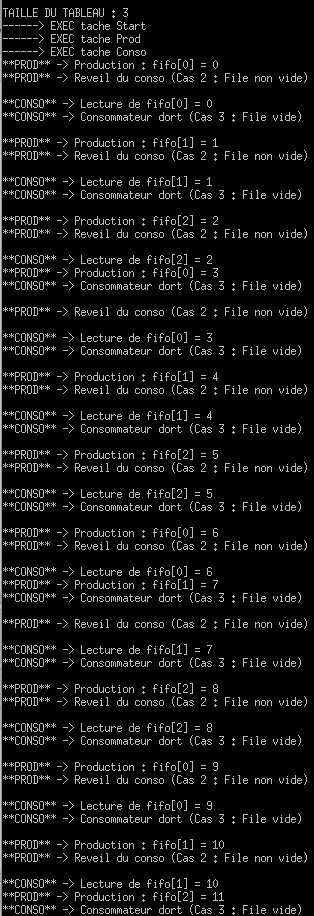
\includegraphics[width=0.4\textwidth]{screens/conso_plus_rapide_sem.png}
		\caption{Consommateur plus rapide que le producteur}
		\label{conso_plus_rapide}
\end{figure}

\newpage

\begin{figure}[h]
	\centering
		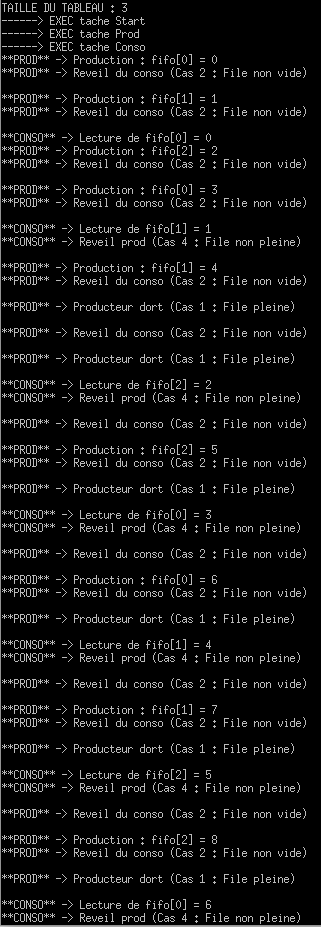
\includegraphics[width=0.4\textwidth]{screens/prod_plus_rapide_sem.png}
		\caption{Producteur plus rapide que le consommateur}
		\label{prod_plus_rapide}
\end{figure}

\newpage

La méthode d'exclusion mutuelle présentée précédemment avec endormissement et réveil des tâches peut poser problème dans le cas général. En effet, nous ne sommes pas à l'abri d'un interblocage des deux tâches si elles sont toutes les deux endormies et qu'elles attendent d'être réveillées. Ceci peut arriver puisque rien ne garantit qu'un signal de réveil ne soit pas interrompue. Une première tâche pourrait en principe envoyer son signal de réveil avant que la seconde tâche s'endorme ce qui engendrerait une attente infinie.

\section{Exercice 2 : Sémaphores}

Un deuxième outil plus efficace que le précédent pour gérer les problèmes de ressources partagées repose sur les sémaphores. Ce mécanisme permet de gérer l'envoi des signaux indépendamment de l'exécution des tâches.

\subsection{Implémentation}

Un sémaphore est composé d'une FIFO de tâches en attente et d'une valeur représentant le nombre de ressources disponibles. Une FIFO est une structure circulaire composée d'une file de tâches, de l'indice de début de la file et de l'indice de fin de la file. Dans cet exercice, nous considérons un tableau de sémaphores. Ci-dessous le fichier header \textit{sem.h} :\newline

\begin{lstlisting}
#ifndef SEM_H_
#define SEM_H_

#include <stdint.h>

#define MAX_SEM 15

typedef struct {
  short taches[MAX_TACHES];
  short debut_file;	
  short fin_file;
} FIFO;

typedef struct {
	FIFO file;     // File circulaire des tâches en attente 
	short valeur ; // compteur du sémaphore e(s) 
} SEMAPHORE ;

void s_init( void );
ushort s_cree( short v );
void s_close( ushort n );
void s_wait( ushort n );
void s_signal ( ushort n );

#endif /* SEM_H_ */
\end{lstlisting}


Un sémaphore se manipule via les cinq fonctions suivantes : \textit{s\_init}, \textit{s\_cree}, \textit{s\_close}, \textit{s\_wait} et \textit{s\_signal}, toutes définies dans le fichier \textbf{sem.c}.\newline

Tout d'abord la fonction \textit{s\_init} permet d'initialiser la valeur de notre tableau de sémaphores. Ici, nous avons choisi d'initialiser toutes nos sémaphores à -1000, nombre que nous considérons, dans cet exercice, inatteignable.\newline

\begin{lstlisting}
SEMAPHORE _sem[MAX_SEM];

void s_init( void )
{
	int i;

	for(i = 0; i < MAX_SEM; i++)
	{
		_sem[i].valeur = -1000;		// non crée
	}
}
\end{lstlisting}

La seconde fonction \textit{s\_cree} nous sert à créer un sémaphore et à l'initialiser à une certaine valeur donnée.\newline

\begin{lstlisting}
ushort s_cree( short v )
{
	int i = 0;

  // si la valeur du sémaphore dépasse le nombre de tâches
	if (v >= MAX_TACHES) 
		return -1;			

	// on cherche un emplacement libre
	while(i<MAX_SEM && _sem[i].valeur != -1000)	
		i++;

	if(i >= MAX_SEM)	// si on n'a pas trouver d'emplacement libre
		return -1;			

	// initialisation du sémaphore à la valeur v
	_sem[i].valeur = v;	
	_sem[i].file.debut_file = 0;	
	_sem[i].file.fin_file = 0;

	return i;
}
\end{lstlisting}

La troisième fonction \textit{s\_close} réinitialise un sémaphore donné. La valeur du sémaphore est remise à -1000 pour qu'on le considère non crée.\newline

\begin{lstlisting}
void s_close( ushort n )
{
	if(n >= MAX_SEM || n < 0)
		return;

	_sem[n].valeur = -1000;
}
\end{lstlisting}

La fonction \textit{s\_wait} implémente l'opération P qui permet de prendre une ressource associée au sémaphore. On décrémente donc la valeur du sémaphore et si celle-ci est strictement inférieure à 0 alors on bloque/endort la tâche ayant effectué la requête et on la met dans la file des tâches en attente associée au sémaphore. Dans notre fonction les tâches sont ajoutées en fin de file.\newline

\begin{lstlisting}
void s_wait( ushort n )
{
	if(n >= MAX_SEM || n < 0)
		return;

	// si le sémaphore n'est pas crée
	if(_sem[n].valeur == -1000)
		return;

	// zone critique car plusieurs tâches ne doivent pas modifier le sémaphore en même temps
	_lock_();			

	_sem[n].valeur--;				// décrémentation du sémaphore

	if(_sem[n].valeur < 0)
	{
		// on ajoute la tâche courante à la fin de la file
		_sem[n].file.taches[_sem[n].file.fin_file] = _tache_c;	
			
		// incrémente la fin de la file
		_sem[n].file.fin_file = _sem[n].file.fin_file + 1;	
			
		// on met à jour la fin de la file circulaire
		// si fin_file < MAX_TACHES alors on ne change rien sinon on revient au début de la file
		_sem[n].file.fin_file = (_sem[n].file.fin_file) % MAX_TACHES; 

		dort();	// la tâche courante s'endort
	}

	_unlock_();
}
\end{lstlisting}

Enfin, la fonction \textit{s\_signal} implémente l'opération V qui permet de libérer une ressource associée au sémaphore. On incrémente donc la valeur du sémaphore et si celle-ci est inférieure ou égale à 0 alors on extrait une tâche de la file des tâches en attente et on la libère/réveille. Dans notre fonction les tâches sont extraites au début de file.\newline

\begin{lstlisting}
void s_signal ( ushort n )
{
	short tache;

	if(n >= MAX_SEM || n < 0)
		return;

	// si le sémaphore n'est pas crée
	if(_sem[n].valeur == -1000)		
		return;

	// zone critique car plusieurs tâches ne doivent pas modifier le sémaphore en même temps
	_lock_();						

	_sem[n].valeur++;				// incrémentation du sémaphore

	if(_sem[n].valeur <= 0)
	{
		// on extrait une tâche au début de la file
		tache = _sem[n].file.taches[_sem[n].file.debut_file]; 	
		
		// incrémente le début de la file
		_sem[n].file.debut_file = _sem[n].file.debut_file + 1;		
		
		// on met à jour le début de la file circulaire
		// si debut_file < MAX_TACHES alors on ne change rien sinon on va à la fin de la file
		_sem[n].file.debut_file = (_sem[n].file.debut_file) % MAX_TACHES; 

		reveille(tache);	// réveil de la tâche
	}

	_unlock_();
}
\end{lstlisting}

\subsection{Producteur/Consommateur}

Afin de tester nos sémaphores, nous avons ré-implémenté le problème du producteur/consommateur en remplaçant les primitives \textit{dort()} et \textit{reveille()} par respectivement \textit{s\_wait} et \textit{s\_signal}. Nous mettons en place deux sémaphores associés respectivement au producteur et au consommateur qu'on initialise à 0. Ceci permet au producteur d'être bloqué si la file est pleine et au consommateur d'être réveillé si il y a un entier à consommer. Le principe reste exactement le même que dans l'exercice précédent. 

\begin{lstlisting}
#define TAILLE_TABLEAU 3	

TACHE tacheStart();
TACHE tacheProd();
TACHE tacheConso();
uint16_t prod, conso;
uint16_t fifo[TAILLE_TABLEAU];	// la file
uint16_t nb_places_libres = TAILLE_TABLEAU;
ushort sem1, sem2;	// sem1 => producteur, sem2 => consommateur

TACHE	tacheStart(void)		// tâche de démarrage
{
  puts("------> EXEC tache Start");
  prod = cree(tacheProd);
  conso = cree(tacheConso);

  active(prod);
  active(conso);

  fin_tache();
}

TACHE	tacheProd(void)		// tâche producteur
{
  puts("------> EXEC tache Prod");

  uint16_t j=0,k,i=0;

  while(1)
  {
	  for (k=0; k<30000; k++);		// producteur plus lent

	  if (nb_places_libres>=1)		// production d'un entier
	  {
		  _lock_();									// zone critique
		  printf("**PROD** -> Production : fifo[%d] = %d\n", i, j);
		  fifo[i]=j;
		  _unlock_();
		  j++;

		  nb_places_libres--;

		  i++;
		  if (i==TAILLE_TABLEAU)	// i = indice de la file
			  i=0;
	  }
	  else			// file pleine
	  {
		  _lock_();
		  puts("**PROD** -> Producteur dort (Cas 1 : File pleine)\n");
		  _unlock_();

		  s_wait(sem1);			// dort()
	  }

	  if (nb_places_libres<TAILLE_TABLEAU)	// file non vide
	  {
		  _lock_();
		  puts("**PROD** -> Reveil du conso (Cas 2 : File non vide)\n");
		  _unlock_();

		  s_signal(sem2);		// reveille(conso);
	  }

  }

  fin_tache();
}

TACHE	tacheConso(void)		// tâche consommateur
{
  uint16_t k,i=0;

  puts("------> EXEC tache Conso");

  s_wait(sem2);			// dort()

  while(1)
  {
	  for (k=0; k<10000; k++);	// consommateur plus rapide

	  if (nb_places_libres==TAILLE_TABLEAU)	// file vide
	  {
		  _lock_();
		  puts("**CONSO** -> Consommateur dort (Cas 3 : File vide)\n");
		  _unlock_();

			s_wait(sem2);		// dort()
	  }
	  else
	  {
		  _lock_();
		  printf("**CONSO** -> Lecture de fifo[%d] = %d\n", i, fifo[i]);
		  _unlock_();

		  nb_places_libres++;

		  i++;
		  if (i==TAILLE_TABLEAU)	// i = indice de la file
			  i=0;
	  }

	  if (nb_places_libres==1)	// file non pleine
	  {
		  _lock_();
		  puts("**CONSO** -> Reveil prod (Cas 4 : File non pleine)\n");
		  _unlock_();

		  s_signal(sem1);			// reveille(prod);
	  }
  }

  fin_tache();
}

int main()
{
  serial_init(115200);
  puts("Test noyau");
  puts("Noyau preemptif");
  puts("*******************DEBUT*********************\n\n\n\n\n");

  printf("TAILLE DU TABLEAU : %d\n", TAILLE_TABLEAU);

  s_init();
  sem1 = s_cree(0);		// prod
  sem2 = s_cree(0);		// conso
  start(tacheStart);
	
  return(0);
}
\end{lstlisting}

Le résultat obtenu lorsque le consommateur est plus rapide que le producteur est exactement le même que sur la figure \ref{conso_plus_rapide}.
De même, dans le cas où le producteur est plus rapide que le consommateur, nous obtenons exactement le même résultat que dans la figure \ref{prod_plus_rapide}.\newline

\subsection{2 Producteurs/ 1 Consommateur}

Nous avons également testé nos sémaphores en ajoutant un producteur au problème précédent. Pour cela, il faut mettre en place un sémaphore binaire ou mutex qu'on initialise à 1 et qui empêche les deux producteurs de produire en même temps. On bloque le mutex avant production et on le libère après. De plus, il faut mettre en place des variables globales pour les indices et les valeurs de la file pour que les producteurs manipulent les mêmes données.\newline

\begin{lstlisting}
#define TAILLE_TABLEAU 3

TACHE tacheStart();
TACHE tacheProd1();
TACHE tacheProd2();
TACHE tacheConso();
uint16_t prod1, prod2, conso;		// 2 producteurs et 1 consommateur
uint16_t fifo[TAILLE_TABLEAU];
uint16_t nb_places_libres = TAILLE_TABLEAU;
ushort sem1, sem2, semMutexProd; 

// variables globales pour les producteurs
// l => indice de la file et j => valeur à cet indice
int l = 0, j = 0; 

TACHE	tacheStart(void)
{
  puts("------> EXEC tache Start");

  prod1 = cree(tacheProd1);
  prod2 = cree(tacheProd2);
  conso = cree(tacheConso);

  active(conso);
  active(prod1);
  active(prod2);

  fin_tache();
}

TACHE	tacheProd1(void)
{
  puts("------> EXEC tache Prod 1");

  uint16_t k;

  while(1)
  {
	  //for (k=0; k<30000; k++);
	  for (k=0; k<10000; k++);

	  s_wait(semMutexProd);	// P du mutex (entrée de la zone critique) 

	  if (nb_places_libres>=1)
	  {
		  _lock_();
		  printf("**PROD 1** -> Production : fifo[%d] = %d\n", l, j);
		  fifo[l]=j;
		  _unlock_();
		  j++;

		  nb_places_libres--;

		  l++;
		  if (l==TAILLE_TABLEAU)
			  l=0;
	  }
	  else
	  {
		  s_wait(sem1);		// dort()
	  }

	  s_signal(semMutexProd);// V du mutex (sortie de la zone critique)


	  if (nb_places_libres<TAILLE_TABLEAU)
	  {
		  s_signal(sem2);		// reveille(conso);
	  }

  }

  fin_tache();
}

TACHE	tacheProd2(void)
{
  puts("------> EXEC tache Prod 2");

  uint16_t k;

  while(1)
  {
	  //for (k=0; k<30000; k++);
	  for (k=0; k<10000; k++);

	  s_wait(semMutexProd); // P du mutex (entrée de la zone critique) 

	  if (nb_places_libres>=1)
	  {
		  _lock_();
		  printf("**PROD 2** -> Production : fifo[%d] = %d\n", l, j);
		  fifo[l]=j;
		  _unlock_();
		  j++;

		  nb_places_libres--;

		  l++;
		  if (l==TAILLE_TABLEAU)
			  l=0;
	  }
	  else
	  {
		  s_wait(sem1);		// dort()
	  }

	  s_signal(semMutexProd);// V du mutex (sortie de la zone critique)

	  if (nb_places_libres<TAILLE_TABLEAU)
	  {
		  s_signal(sem2);		// reveille(conso);
	  }

  }

  fin_tache();
}

TACHE	tacheConso(void)
{
  uint16_t k,i=0;

  puts("------> EXEC tache Conso");

  s_wait(sem2);	// dort()

  while(1)
  {
	  for (k=0; k<30000; k++);
	  //for (k=0; k<10000; k++);

	  if (nb_places_libres==TAILLE_TABLEAU)
	  {
		  s_wait(sem2);	// dort()
	  }
	  else
	  {
		  _lock_();
		  printf("**CONSO** -> Lecture de fifo[%d] = %d\n", i, fifo[i]);
		  _unlock_();

		  nb_places_libres++;

		  i++;
		  if (i==TAILLE_TABLEAU)
			  i=0;
	  }

	  if (nb_places_libres==1)
	  {
		  s_signal(sem1);	// reveille(prod);
	  }

  }

  fin_tache();
}

int main()
{
  serial_init(115200);
  puts("Test noyau");
  puts("Noyau preemptif");
  puts("*******************DEBUT*********************\n\n\n\n\n");

  printf("TAILLE DU TABLEAU : %d\n", TAILLE_TABLEAU);

  s_init();
  sem1 = s_cree(0);		// prod
  sem2 = s_cree(0);		// conso
	
	// mutex entre les 2 producteurs pour les empêcher de produire en même temps
  semMutexProd = s_cree(1);	
		
  start(tacheStart);

  return(0);
}
\end{lstlisting}

Nous avons testé deux configurations, l'une où les producteurs sont plus rapides que le consommateur et la deuxième où le consommateur est plus rapide que les producteurs. On suppose que les producteurs ont la même vitesse.\newline

Le résultat dans le premier cas est visible sur la figure \ref{prod_plus_rapide_sem_2prod_meme_vitesse_1conso}. 
On voit bien dans ce cas que le producteur 1 et 2 ne produisent pas en même temps mais à tour de rôle. Comme le consommateur est plus lent il consomme les entiers avec un retard de 2 indices. Par exemple, le producteur 2 écrit l'entier 2 à la case 2 et juste après le consommateur lit l'entier 0 à la case 0 (2 écritures ont été faite entre temps à cause de la rapidité des producteurs).\newline

Dans le cas où le consommateur est plus rapide (figure \ref{conso_plus_rapide_sem_2prod_meme_vitesse_1conso}), on remarque qu'il n'a pas de retard, il consomme les entiers directement après production ce qui est tout à fait cohérent.

\newpage

\begin{figure}[h]
	\centering
		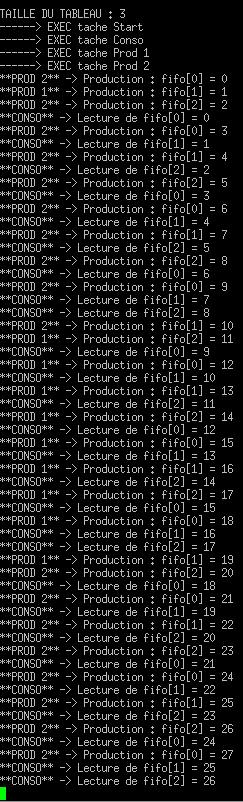
\includegraphics[width=0.4\textwidth]{screens/prod_plus_rapide_sem_2prod_meme_vitesse_1conso.png}
		\caption{2 producteurs plus rapide que le consommateur}
		\label{prod_plus_rapide_sem_2prod_meme_vitesse_1conso}
\end{figure}

\newpage

\begin{figure}[h]
	\centering
		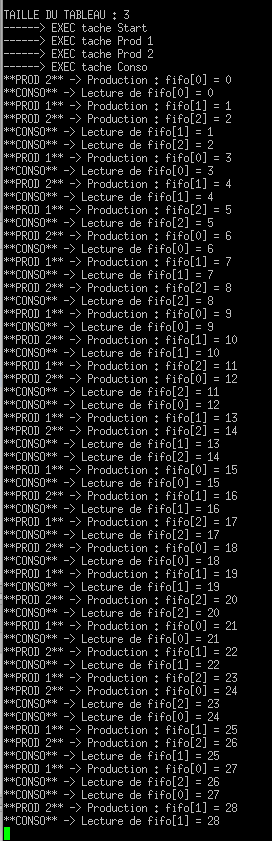
\includegraphics[width=0.4\textwidth]{screens/conso_plus_rapide_sem_2prod_meme_vitesse_1conso.png}
		\caption{Consommateur plus rapide que les 2 producteurs}
		\label{conso_plus_rapide_sem_2prod_meme_vitesse_1conso}
\end{figure}

\newpage

\subsection{1 Producteur/ 2 Consommateurs}

Nous avons également testé le cas opposé où il y a cette fois-ci un producteur et deux consommateurs. Le principe est exactement le même que précédemment sauf que le mutex s'applique aux deux consommateurs avant et après lecture d'un entier. De même que précédemment, les consommateurs partagent des variables globales. On suppose que les consommateurs ont la même vitesse.\newline

\begin{lstlisting}
#define TAILLE_TABLEAU 3

TACHE tacheStart();
TACHE tacheProd();
TACHE tacheConso1();
TACHE tacheConso2();
uint16_t prod, conso1, conso2;		// 2 conso et 1 prod
uint16_t fifo[TAILLE_TABLEAU];
uint16_t nb_places_libres = TAILLE_TABLEAU;
ushort sem1, sem2, semMutexConso;

// variables globales pour les producteurs
// l => indice de la file et j => valeur à cet indice
int l = 0, j = 0;

TACHE	tacheStart(void)
{
  puts("------> EXEC tache Start");

  prod = cree(tacheProd);
  conso1 = cree(tacheConso1);
  conso2 = cree(tacheConso2);

  active(conso1);
  active(conso2);
  active(prod);

  fin_tache();
}

TACHE	tacheProd(void)
{
  puts("------> EXEC tache Prod");

  uint16_t j=0,k,i=0;

  while(1)
  {
	  for (k=0; k<30000; k++);
	  //for (k=0; k<10000; k++);

	  if (nb_places_libres>=1)
	  {
		  _lock_();
		  printf("**PROD** -> Production : fifo[%d] = %d\n", i, j);
		  fifo[i]=j;
		  _unlock_();
		  j++;

		  nb_places_libres--;

		  i++;
		  if (i==TAILLE_TABLEAU)
			  i=0;
	  }
	  else
	  {
		  s_wait(sem1);		// dort()
	  }

	  if (nb_places_libres<TAILLE_TABLEAU)
	  {
		  s_signal(sem2);		// reveille(conso);
	  }

  }

  fin_tache();
}


TACHE	tacheConso1(void)
{
  uint16_t k;

  puts("------> EXEC tache Conso 1");

  s_wait(sem2);	// dort()

  while(1)
  {
	  //for (k=0; k<30000; k++);
	  for (k=0; k<10000; k++);


	  s_wait(semMutexConso); // P du mutex (entrée de la zone critique) 

	  if (nb_places_libres==TAILLE_TABLEAU)
	  {
		  s_wait(sem2);	// dort()
	  }
	  else
	  {
		  _lock_();
		 printf("**CONSO 1** -> Lecture de fifo[%d] = %d\n", l, fifo[l]);
		  _unlock_();

		  nb_places_libres++;

		  l++;
		  if (l==TAILLE_TABLEAU)
			  l=0;
	  }

	  s_signal(semMutexConso);// V du mutex (sortie de la zone critique)

	  if (nb_places_libres==1)
	  {
		  s_signal(sem1);	// reveille(prod);
	  }

  }

  fin_tache();
}

TACHE	tacheConso2(void)
{
  uint16_t k;

  puts("------> EXEC tache Conso 2");

  s_wait(sem2);	// dort()

  while(1)
  {
	  //for (k=0; k<30000; k++);
	  for (k=0; k<10000; k++);


	  s_wait(semMutexConso); // P du mutex (entrée de la zone critique) 

	  if (nb_places_libres==TAILLE_TABLEAU)
	  {
		  s_wait(sem2);	// dort()
	  }
	  else
	  {
		  _lock_();
		  printf("**CONSO 2** -> Lecture de fifo[%d] = %d\n",l, fifo[l]);
		  _unlock_();

		  nb_places_libres++;

		  l++;
		  if (l==TAILLE_TABLEAU)
			  l=0;
	  }

	  s_signal(semMutexConso);// V du mutex (sortie de la zone critique)


	  if (nb_places_libres==1)
	  {
		  s_signal(sem1);	// reveille(prod);
	  }

  }

  fin_tache();
}

int main()
{
  serial_init(115200);
  puts("Test noyau");
  puts("Noyau preemptif");
  puts("*******************DEBUT*********************\n\n\n\n\n");

  printf("TAILLE DU TABLEAU : %d\n", TAILLE_TABLEAU);

  s_init();
  sem1 = s_cree(0);		// prod
  sem2 = s_cree(0);		// conso
	
	// mutex entre les 2 consommateurs pour les empêcher de consommer en même temps
  semMutexConso = s_cree(1);		
	
  start(tacheStart);

  return(0);
}
\end{lstlisting}

Le résultat dans le cas où le producteur est plus rapide que les consommateurs est visible sur la figure \ref{prod_plus_rapide_sem_2conso_meme_vitesse_1prod}. Les consommateurs ont tendance à être en retard d'un ou deux indices.\newline
Pour le cas où les consommateurs sont plus rapides que le producteur (figure \ref{conso_plus_rapide_sem_2conso_meme_vitesse_1prod}), la consommation se fait dans l'ordre juste après les productions comme précédemment.

\newpage

\begin{figure}[h]
	\centering
		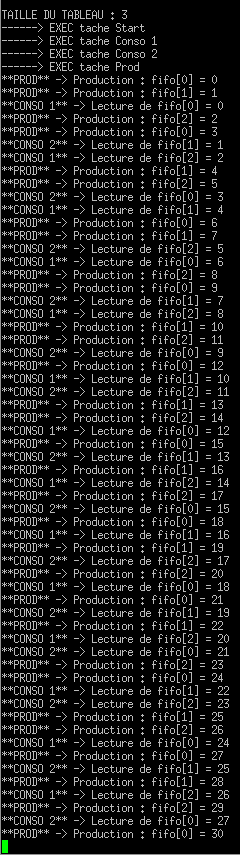
\includegraphics[width=0.35\textwidth]{screens/prod_plus_rapide_sem_2conso_meme_vitesse_1prod.png}
		\caption{Producteur plus rapide que les 2 consommateurs}
		\label{prod_plus_rapide_sem_2conso_meme_vitesse_1prod}
\end{figure}

\newpage

\begin{figure}[h]
	\centering
		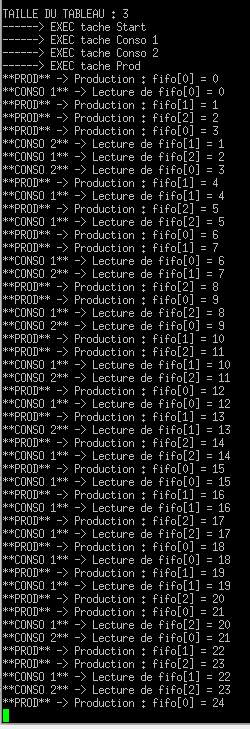
\includegraphics[width=0.4\textwidth]{screens/conso_plus_rapide_sem_2conso_meme_vitesse_1prod.png}
		\caption{2 consommateurs plus rapide que le producteur}
		\label{conso_plus_rapide_sem_2conso_meme_vitesse_1prod}
\end{figure}

\newpage

\subsection{2 Producteurs/ 2 Consommateurs}

Finalement, nous avons implémenté le cas avec 2 producteurs et 2 consommateurs. Dans cette exemple, nous avons besoin des 2 mutex précédents, un pour empêcher les producteurs de produire en même temps et un autre pour empêcher les consommateurs de produire en même temps. Les producteurs partagent également des variables globales pour la file d'entiers et de même pour les consommateurs. Le principe reste exactement le même que précédemment.\newline

\begin{lstlisting}
#define TAILLE_TABLEAU 3

TACHE tacheStart();
TACHE tacheProd1();
TACHE tacheProd2();
TACHE tacheConso1();
TACHE tacheConso2();
uint16_t prod1, prod2, conso1, conso2;		// 2 conso et 2 prod
uint16_t fifo[TAILLE_TABLEAU];
uint16_t nb_places_libres = TAILLE_TABLEAU;
ushort sem1, sem2, semMutexConso, semMutexProd;

// variables globales pour les producteurs et consommateurs
int l = 0, j = 0, m = 0;


TACHE	tacheStart(void)
{
  puts("------> EXEC tache Start");

  prod1 = cree(tacheProd1);
  prod2 = cree(tacheProd2);
  conso1 = cree(tacheConso1);
  conso2 = cree(tacheConso2);

  active(conso1);
  active(conso2);
  active(prod1);
  active(prod2);

  fin_tache();
}

TACHE	tacheProd1(void)
{
  puts("------> EXEC tache Prod 1");

  uint16_t k;

  while(1)
  {
	  for (k=0; k<30000; k++);
	  //for (k=0; k<10000; k++);

	  s_wait(semMutexProd);// P du mutex (entrée de la zone critique)

	  if (nb_places_libres>=1)
	  {
		  _lock_();
		  printf("**PROD 1** -> Production : fifo[%d] = %d\n", l, j);
		  fifo[l]=j;
		  _unlock_();
		  j++;

		  nb_places_libres--;

		  l++;
		  if (l==TAILLE_TABLEAU)
			  l=0;
	  }
	  else
	  {
		  s_wait(sem1);		// dort()
	  }

	  s_signal(semMutexProd);// V du mutex (sortie de la zone critique)


	  if (nb_places_libres<TAILLE_TABLEAU)
	  {
		  s_signal(sem2);		// reveille(conso);
	  }

  }

  fin_tache();
}

TACHE	tacheProd2(void)
{
  puts("------> EXEC tache Prod 2");

  uint16_t k;

  while(1)
  {
	  for (k=0; k<30000; k++);
	  //for (k=0; k<10000; k++);

	  s_wait(semMutexProd);// P du mutex (entrée de la zone critique)

	  if (nb_places_libres>=1)
	  {
		  _lock_();
		  printf("**PROD 2** -> Production : fifo[%d] = %d\n", l, j);
		  fifo[l]=j;
		  _unlock_();
		  j++;

		  nb_places_libres--;

		  l++;
		  if (l==TAILLE_TABLEAU)
			  l=0;

	  }
	  else
	  {
		  s_wait(sem1);		// dort()
	  }

	  s_signal(semMutexProd);// V du mutex (sortie de la zone critique)

	  if (nb_places_libres<TAILLE_TABLEAU)
	  {
		  s_signal(sem2);		// reveille(conso);
	  }

  }

  fin_tache();
}


TACHE	tacheConso1(void)
{
  uint16_t k;

  puts("------> EXEC tache Conso 1");

  s_wait(sem2);	// dort()

  while(1)
  {
	  //for (k=0; k<30000; k++);
	  for (k=0; k<10000; k++);


	  s_wait(semMutexConso); // P du mutex (entrée de la zone critique)

	  if (nb_places_libres==TAILLE_TABLEAU)
	  {
		  s_wait(sem2);	// dort()
	  }
	  else
	  {
		  _lock_();
		 printf("**CONSO 1** -> Lecture de fifo[%d] = %d\n", m, fifo[m]);
		  _unlock_();

		  nb_places_libres++;

		  m++;
		  if (m==TAILLE_TABLEAU)
			  m=0;
	  }

	  s_signal(semMutexConso);// V du mutex (sortie de la zone critique)

	  if (nb_places_libres==1)
	  {
		  s_signal(sem1);	// reveille(prod);
	  }

  }

  fin_tache();
}

TACHE	tacheConso2(void)
{
  uint16_t k;

  puts("------> EXEC tache Conso 2");

  s_wait(sem2);	// dort()

  while(1)
  {
	  //for (k=0; k<30000; k++);
	  for (k=0; k<10000; k++);

	  s_wait(semMutexConso); // P du mutex (entrée de la zone critique)

	  if (nb_places_libres==TAILLE_TABLEAU)
	  {
		  s_wait(sem2);	// dort()
	  }
	  else
	  {
		  _lock_();
		  printf("**CONSO 2** -> Lecture de fifo[%d] = %d\n",m, fifo[m]);
		  _unlock_();

		  nb_places_libres++;

		  m++;
		  if (m==TAILLE_TABLEAU)
			  m=0;
	  }

	  s_signal(semMutexConso);// V du mutex (sortie de la zone critique)


	  if (nb_places_libres==1)
	  {
		  s_signal(sem1);	// reveille(prod);
	  }

  }

  fin_tache();
}

int main()
{
  serial_init(115200);
  puts("Test noyau");
  puts("Noyau preemptif");
  puts("*******************DEBUT*********************\n\n\n\n\n");

  printf("TAILLE DU TABLEAU : %d\n", TAILLE_TABLEAU);

  s_init();
  sem1 = s_cree(0);		// prod
  sem2 = s_cree(0);		// conso
  
  // mutex entre les 2 consommateurs pour les empêcher de consommer en même temps
  semMutexConso = s_cree(1);
  
  // mutex entre les 2 producteurs pour les empêcher de produire en même temps
  semMutexProd = s_cree(1);		

  start(tacheStart);

  return(0);
}
\end{lstlisting}

Pour cette exemple, nous avons testé trois configurations différentes :\newline 

1) Les producteurs et consommateurs ont tous la même vitesse (figure \ref{prod_conso_meme_vitesse_sem_2prod_meme_vitesse_2conso_meme_vitesse_TRAFIK}).

2) Les producteurs ont la même vitesse mais sont plus rapides que les consommateurs qui ont la même vitesse également (figure \ref{prod_plus_rapide_sem_2prod_meme_vitesse_2conso_meme_vitesse_TRAFIK}).

3) Les consommateurs ont la même vitesse mais sont plus rapides que les producteurs qui ont la même vitesse également (figure \ref{conso_plus_rapide_sem_2prod_meme_vitesse_2conso_meme_vitesse}).



\newpage

\begin{figure}[h]
	\centering
		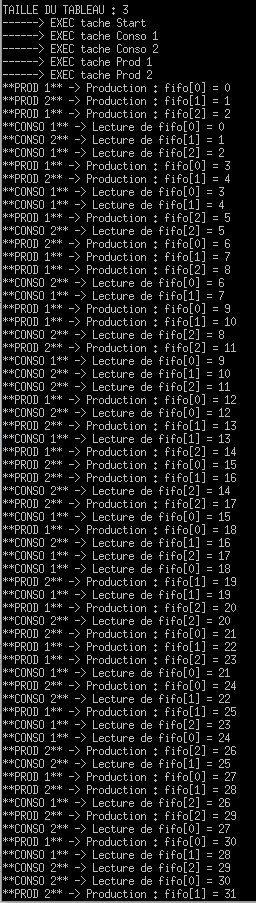
\includegraphics[width=0.35\textwidth]{screens/prod_conso_meme_vitesse_sem_2prod_meme_vitesse_2conso_meme_vitesse_TRAFIK.png}
		\caption{2 producteurs et 2 consommateurs à la même vitesse}
		\label{prod_conso_meme_vitesse_sem_2prod_meme_vitesse_2conso_meme_vitesse_TRAFIK}
\end{figure}

\newpage

\begin{figure}[h]
	\centering
		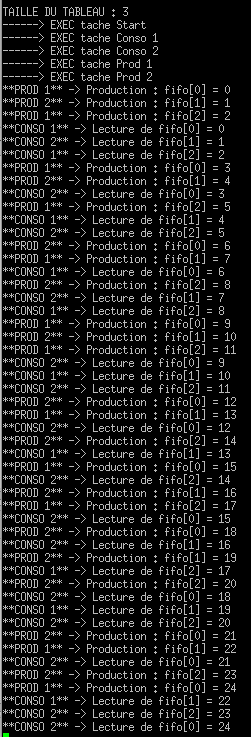
\includegraphics[width=0.4\textwidth]{screens/prod_plus_rapide_sem_2prod_meme_vitesse_2conso_meme_vitesse_TRAFIK.png}
		\caption{2 producteurs plus rapides que les 2 consommateurs}
		\label{prod_plus_rapide_sem_2prod_meme_vitesse_2conso_meme_vitesse_TRAFIK}
\end{figure}

\newpage

\begin{figure}[h]
	\centering
		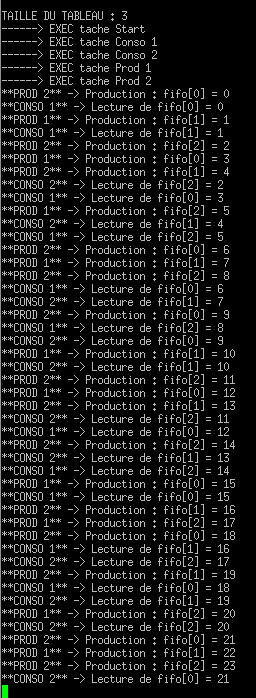
\includegraphics[width=0.4\textwidth]{screens/conso_plus_rapide_sem_2prod_meme_vitesse_2conso_meme_vitesse.png}
		\caption{2 consommateurs plus rapides que les 2 producteurs}
		\label{conso_plus_rapide_sem_2prod_meme_vitesse_2conso_meme_vitesse}
\end{figure}

\newpage






\chapter{Rapport TP3 - Parties 5 et 6}
\section{5ème partie : Le dîner des philosophes}

Le dîner des philosophes est un problème de synchronisation très connu. Cinq philosophes sont réunis autour d'une table circulaire pour dîner. Cinq couverts composés d'une assiette et d'une fourchette sont disposés autour de la table. Chaque philosophe a besoin de deux fourchettes pour manger son plat, la fourchette de gauche et la fourchette de droite. 
Un philosophe ne peut être que dans trois états, soit il pense, soit il a faim, soit il mange.
On suppose dans notre cas que les fourchettes sont numérotées de 0 à 4 et que les philosophes sont numérotées de 1 à 5. Ainsi, le philosophe numéro 1 aura besoin de la fourchette 0 à sa gauche et de la fourchette 1 à sa droite, et le philosophe 5 aura besoin de la fourchette 4 à sa gauche et de la fourchette 0 à sa droite.

\begin{figure}[h]
	\centering
		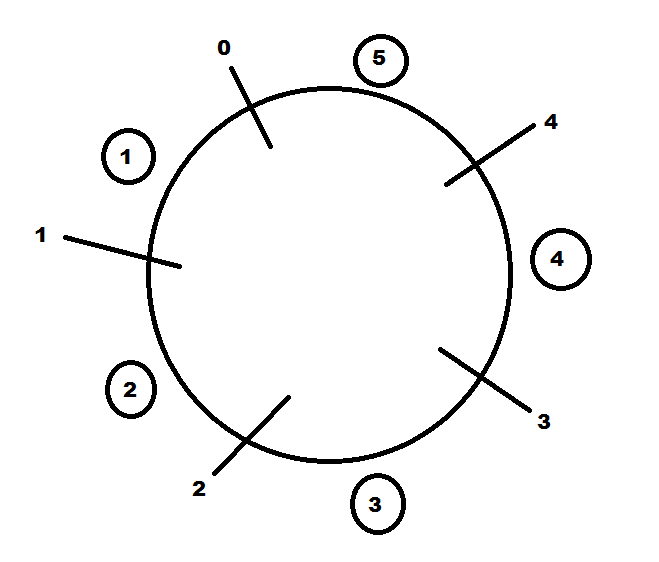
\includegraphics[width=0.6\textwidth]{screens/philo_table.png}
		\caption{La table des philosophes}
\end{figure}

\newpage

Nous avons résolu ce problème à l'aide des sémaphores suivants :\newline

1) Un tableau de 5 sémaphores initialisés à 1 pour l'accès aux fourchettes. Un sémaphore à 1 signifie que la fourchette est disponible et 0 qu'elle n'est pas disponible.\newline
2) Un sémaphore initialisé à 4 qui garanti qu'une fourchette sera toujours disponible. En effet, normalement il n'est pas judicieux de mettre des sémaphores sur les fourchettes car ceci peut générer un interblocage si jamais les philosophes s'emparent tous de la fourchette gauche ou de la fourchette droite. C'est pour cela que nous avons ajouté un sémaphore qui autorise ou non la prise d'une fourchette. Comme ce sémaphore est initialisé à 4, il autorise au maximum la prise de 4 fourchettes donc il restera toujours une fourchette de disponible.\newline
3) Un sémaphore d'attente initialisé à 0 qui permet à chaque philosophe qui a fini de manger d'attendre la fin des autres. Lorsqu'un philosophe fini de manger, il se bloque sur ce sémaphore. Ceci permet de finir proprement le repas. On suppose ici que chaque philosophe n'a qu'un plat et qu'il n'y a pas de second repas.\newline
4) Un sémaphore de type mutex initialisé à 1 qui permet de protéger la variable qui compte le nombre de philosophes ayant fini de manger.\newline

En résumé, un philosophe pense puis lorsqu'il a faim il demande au sémaphore numéro 2 s'il peut prendre une fourchette. Si oui, c'est à dire s'il reste au moins deux fourchettes, alors il demande au tableau de sémaphores numéro 1 s'il peut s'emparer de la fourchette de gauche et de droite. La fourchette de gauche associé à ce philosophe se trouve à l'indice $(id - 1) \% 5$ avec $id$ l'identifiant du philosophe et la fourchette de droite se trouve à l'indice $id \% 5$. Par exemple, le philosophe 5 tentera de s'emparer de la fourchette $(5 - 1) \% 5 = 4 \% 5 = 4$ à sa gauche et de la fourchette $id \% 5 = 5 \% 5 = 0$ à sa droite.
Si le philosophe a pris ses deux fourchettes, alors il mange et lorsqu'il a terminé, il libère le sémaphore numéro 2, c'est à dire qu'il incrémente le nombre de fourchettes que tous les philosophes peuvent prendre en même temps. Il libère aussi les sémaphores associés aux fourchettes qu'il vient d'utiliser via le tableau de sémaphores numéro 1.
Puis il demande au mutex numéro 4 s'il peut incrémenter la variable qui compte le nombre de philosophes ayant fini de manger. Si oui, alors il y a deux cas possibles, soit la variable est inférieure à 5 ce qui veut dire que des philosophes n'ont pas encore fini de manger, soit elle vaut 5 ce qui veut dire que tout le monde a fini de manger. Dans le premier cas, le philosophe se bloque sur le sémaphore d'attente numéro 3 pour attendre ses collègues et dans le deuxième cas, tous les philosophes sont libérés et c'est la fin du repas.

\newpage

\begin{lstlisting}
TACHE tacheStart();
TACHE tachePhilo();

// semProtectFourch => garanti qu'une fourchette sera toujours disponible
// semAttente => permet à chaque philosophe qui a fini de manger d'attendre la fin des autres
// mutex => protéger la variable qui compte le nombre de philosophes ayant fini de manger
ushort semProtectFourch, semAttente, mutex;	

// tableau de sémaphores des fourchettes
ushort semFourchette[5];	

ushort id_philo;	// id unique par philosophe

// variable qui compte le nombre de philosophes ayant fini de manger
int j;	

TACHE	tacheStart(void)
{
		puts("------> EXEC tache Start");

    int i;
    s_init();	// initialisation des sémaphores

		// autorise au maximum la prise de 4 fourchettes
    semProtectFourch = s_cree(4);			

		mutex = s_cree(1);
		semAttente = s_cree(0);

    for(i=0; i < 5; i++) 
        semFourchette[i] = s_cree(1);

    for(id_philo=0; id_philo < 5; id_philo++)
    	active(cree(tachePhilo));
    
		fin_tache();
}

TACHE tachePhilo()
{
	uint16_t k;

	ushort id = id_philo; // récupération de l'id du philosophe
  printf("------> Philosophe n° : %d demarre\n", id); // il pense

  while (1)
	{
    for (k=0; k<60000; k++);	// il pense

		_lock_();
    printf("------> Philosophe n° : %d attend pour manger : il a faim\n", id);
    _unlock_();

		// autoriser à prendre une fourchette ?
    s_wait(semProtectFourch); 
		
		// on prend la fourchette de gauche
    s_wait(semFourchette[ (id - 1) % 5 ]);
			
		// on prend la fourchette de droite
    s_wait(semFourchette[ id % 5 ]);	

		_lock_();
    printf("------> Philosophe n° : %d en train de manger\n", id);
    _unlock_();

		for (k=0; k<30000; k++);		// temps d'attente pour qu'il mange

		_lock_();
    printf("------> Philosophe n° : %d a fini de manger : il pense\n", id);
    _unlock_();

		// autorisation de prendre une fourchette de plus
		s_signal(semProtectFourch);
		
		// on depose la fourchette de gauche
    s_signal(semFourchette[ (id - 1) % 5 ]); 
		
		// on depose la fourchette de droite
    s_signal(semFourchette[ id % 5 ]);	


		s_wait(mutex);		// pour protéger le compteur j
		j++;	 // un philosophe de plus a fini de manger

		if(j == 5) 			// ils ont tous fini de manger
		{
			for(k=0; k < 5; k++)
			s_signal(semAttente);	// on libere toutes les tâches 

			j = 0;						
			s_signal(mutex);

	    printf("------> Fin du repas\n", id);

			fin_tache();		
		}
		else
		{
			s_signal(mutex);
			s_wait(semAttente);	// on bloque la tâche, le philosophe attend 

			fin_tache();	// fin du repas
		}

  }
}

int main()
{
  serial_init(115200);
  puts("Test noyau");
  puts("Noyau preemptif");
  puts("*******************DEBUT*********************\n\n\n\n\n");

  start(tacheStart);

  return(0);
}
\end{lstlisting}


\begin{figure}[h]
	\centering
		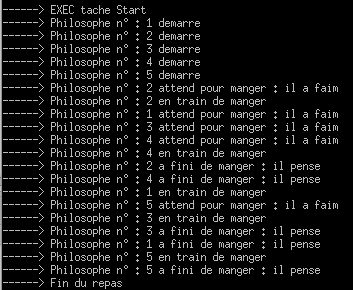
\includegraphics[width=0.5\textwidth]{screens/philo_pense_meme_vitesse.png}
		\caption{Le dîner des philosophes}
\end{figure}

\newpage

On voit bien sur la figure précédente que lorsque le philosophe 2 mange, les philosophes 1 et 3 sont logiquement bloqués. Seul le philosophe 4 est autorisé à manger en même que le philosophe 2. De même, lorsque le philosophe 1 mange, seul le philosophe 3 peut manger en même temps sachant que les philosophes 2 et 4 ont fini de manger et que le philosophe 5 est bloqué. Enfin, lorsque le philosophe 5 a fini de manger, le repas se termine.

\section{6ème partie : Communication par tubes}
Dans cette partie nous devons réaliser un système de communication par tube. De chaque côté du tube ne se trouve qu'une seule et unique tâche.

Commençons par le fichier \textit{pipe.h} :
\begin{lstlisting}
#ifndef PIPE_H_
#define PIPE_H_

#include "noyau.h"

#define MAX_PIPES 5 //Nombre de tubes
#define SIZE_PIPE 10 //Taille de chaque tube

typedef struct
{
	ushort pr_w , pr_r ; // redacteur & lecteur du tube  
	ushort ocupp ;  // donnees restantes  
	uchar is, ie ;    // pointeurs d?entree / sortie  
	uchar tube[SIZE_PIPE] ; // Tampon  
} PIPE;

PIPE  _pipe[MAX_PIPES] ;   // Variables tubes  


//Allocation du conduit
unsigned int p_open(unsigned int redacteur, unsigned int lecteur); 
//Libération du tube
void p_close (unsigned int conduit); 
//Lecture dans un tube
void p_read  (int tube, uchar* donnees, int quantite); 
//Ecriture dans un tube
void p_write(int tube, uchar* donnees, int quantite); 
//Initialisation des tubes
void init_pipes();
\end{lstlisting}

Nous avons choisi un nombre de tubes égal à 5 et une taille de 10 pour chaque tube.

\subsection{Fonction init\_pipes}
\begin{lstlisting}
void init_pipes()
{
	unsigned int i;
	for (i=0;i<MAX_PIPES;i++)
		_pipe[i].pr_w=MAX_TACHES; //Tube inutilisé
}
\end{lstlisting}
La fonction \textit{init\_pipes()} initialise tous les tubes au départ en leur assignant la constante MAX\_TACHES comme écrivain, ce qui signifie qu'ils sont inutilisés.

\subsection{Fonction p\_open}
\begin{lstlisting}
//Ouvre un nouveau pipe
unsigned int p_open(unsigned int redacteur, unsigned int lecteur)
{
	//VérifIier si les tâches sont créées
	if (_contexte[redacteur].status == NCREE || _contexte[lecteur].status == NCREE)
		return -1;

	//Vérifier qu'il n'existe pas de tube avec ces 2 taches
	unsigned int i;
	for (i=0 ; i<MAX_PIPES ; i++)
	{
		if (_pipe[i].pr_w == redacteur && _pipe[i].pr_r == lecteur)
			//Il existe un tube avec ces 2 taches
			return -1;
	}

	//Trouver un tube non utilisé
	i=0;
	while ( (_pipe[i].pr_w != MAX_TACHES) && (i < MAX_PIPES) )
		i++;
	if (i == MAX_PIPES) //Aucun tube n'est libre
		return -2;

	//Initialisation du tube
	_pipe[i].pr_w = redacteur;
	_pipe[i].pr_r = lecteur;
	_pipe[i].is = _pipe[i].ie = 0;
	_pipe[i].ocupp = 0; //Données restantes (0 au départ)


	//Retourner le numéro du tube créé
	return i;
}
\end{lstlisting}

Cette fonction permet d'ouvrir un nouveau tube. Elle prend comme arguments la tâche lectrice et la tâche rédactrice. 

On commence par vérifier si ces deux tâches existent, et qu'il n'existe pas déjà de tube entre ces deux tâches. Ensuite, on cherche un tube non utilisé dans le tableau de tube \textit{\_pipe}. Une fois trouvé, on attribue les valeurs adéquates aux champs pr\_w, pr\_r, is, ie (tous les deux à zéro) et occup (à zéro aussi) du tube.


\subsection{Fonction p\_close}
\begin{lstlisting}
//Ferme un pipe
void p_close (unsigned int conduit)
{
	_pipe[conduit].pr_w = MAX_TACHES;
}
\end{lstlisting}
La fonction \textit{p\_close} permet de fermer un tube en le rendant inutilisé en attribuant la valeur MAX\_TACHES à son écrivain.


\subsection{Fonction p\_read}
\begin{lstlisting}
//Lit un certain nombre de données sur un pipe
void p_read  (int tube, uchar* donnees, int quantite)
{
	//Vérifier que le tube existe et que la tâche en est propriétaire
	if ( (_pipe[tube].pr_r != _tache_c) )
	{
		printf("Tache non autorisee a lire dans le pipe\n");
		return;
	}

	//Lire les données à partir du tampon
	int i = 0;
	for (i=0 ; i < quantite ; i++)
	{
		//Vérifier que le tampon n?est pas vide, sinon endormir la tache
		if (_pipe[tube].ocupp == 0)
		{
			printf("Tampon vide ==> endormissement de la tache %d\n", _pipe[tube].pr_r);
			dort();
		}

		donnees[i] = _pipe[tube].tube[_pipe[tube].is];
		_pipe[tube].is++;
		_pipe[tube].ocupp--;

		//Si  le  tube  était  plein  et  si
		//la  tâche  écrivain  est  suspendue	sur  une
		//écriture  dans  ce  tube alors la réveiller 
		if ( (_pipe[tube].ocupp+1 == SIZE_PIPE) && (_contexte[_pipe[tube].pr_w].status == SUSP) )
			reveille(_pipe[tube].pr_w);
	}
}
\end{lstlisting}

La fonction \textit{p\_read} lit une certaine quantité de données sur un tube. Elle prend comme argument le tube en question, un tableau de données et la quantité à lire.

On commence une fois de plus par une vérification. On vérifie si le tube demandé existe et si la tâche qui veut y lire en a bien le droit (c'est à dire on vérifie si le champ pr\_r du tube est bien la tâche courante).

Ensuite, on peut commencer à lire les données du tube. Sachant que nos tubes sont des tableaux de caractères et qu'on lit une certaine quantité, on fait une boucle allant de 0 à cette quantité pour lire caractère par caractère.

A chaque lecture du tube, on vérifie s'il est vide ou non. S'il l'est, on l'endort. Sinon, on peut procéder à la lecture du caractère (à l'emplacement de sortie "is"). On incrémente le champ \textit{is} du tube et on décrémente la champ \textit{ocupp} car on vient de lire un caractère.

Enfin, si  le  tube  était  plein  et  si la  tâche  écrivain  est  suspendue sur une écriture dans ce tube (c'est à dire si l'écrivain, lors d'une tentation d'écriture est tombé sur un tube plein) alors on la réveille. De cette façon, une écriture sur un tube plein ne posera pas de problème : le rédacteur attendra simplement (en s'endormant) que le lecteur lise une donnée dans le tube et le réveille.



\subsection{Fonction p\_write}
\begin{lstlisting}
//Ecrit un certain nombre de données sur un pipe
void p_write(int tube, uchar* donnees, int quantite)
{
	//Vérifier que le tube existe et que la tâche en est propriétaire
	if ( (_pipe[tube].pr_w != _tache_c) )
	{
		printf("Tache non autorisee a ecrire dans le pipe\n");
		return;
	}

	//Copie des données dans le tube
	int i;
	for (i=0 ; i < quantite ; i++)
	{
		//Vérifier qu?il y a de la place dans le tampon, sinon endormir la tache
		if (_pipe[tube].ocupp == SIZE_PIPE)
		{
			printf("Plus de place dans le tampon ==> endormissement de la tache %d\n", _pipe[tube].pr_w);
			dort();
		}

		//Copie des données
		_pipe[tube].tube[_pipe[tube].ie] = donnees[i];
		_pipe[tube].ie++;
		_pipe[tube].ocupp++;

		//Si le tube était vide et si
		//la tache lectrice est suspendue sur
		//une lecture de ce tube alors la réveiller
		if ( (_pipe[tube].ocupp-1 == 0) && (_contexte[_pipe[tube].pr_r].status == SUSP) )
			reveille(_pipe[tube].pr_r);
	}

}
\end{lstlisting}

La fonction \textit{p\_write} écrit une certaine quantité de données sur un tube.  Elle prend en argument le tube désiré, un tableau de données et une quantité de données à écrire.

Tout comme pour la lecture, on vérifie si le tube demandé existe et si la tâche qui veut y écrire en a bien le droit (c'est à dire on vérifie si le champ pr\_w du tube est bien la tâche courante).

On peut ensuite commencer à écrire dans le tube. On procède de la même manière que la lecture c'est à dire caractère par caractère.

Si le tube est plein, on endort le rédacteur jusqu'à ce que le lecteur le réveille après avoir lu un caractère. Sinon, on peut copier le caractère dans le tube (à l'emplacement d'entrée "ie"). On incrémente ie et ocupp comme il se doit.

Enfin, si le tube était vide et si la tache lectrice est suspendue sur une lecture de ce tube (c'est à dire si un lecteur, en tentant de lire, est tombé sur un tube vide) alors on la réveille. De cette façon, une lecture sur un tube vide ne posera pas de problème : le lecteur attendra simplement (en s'endormant) que le rédacteur écrive dans le tube et le réveille.

\subsection{Test de ces fonctions}
Pour tester notre système de tubes, on réalise un programme de deux tâches : la tâche A et la tâche B. Deux tubes leur sont associés : un de A vers B et l'autre de B vers A. Le déroulement du programme est le suivant :
\begin{itemize}
\item La tâche A envoie le message "salut" à la tâche B via le premier tube
\item La tâche B reçoit ce message via ce même tube
\item La tâche B envoie ce message reçu à la tâche A via le deuxième tube
\item La tâche A reçoit le message via le deuxième tube.
\end{itemize}

Voici le code associé :

\begin{lstlisting}
#include "pipe.h"
#include "noyau.h"
#define TAILLE_MESSAGE 10

//definitions des fonctions citées précédemment

TACHE tacheStart();
TACHE tacheA();
TACHE tacheB();
uint16_t tA, tB;
int pipe1, pipe2;

TACHE	tacheStart(void)
{
  puts("------> EXEC tache Start");

  init_pipes();
  puts("Pipes initialises\n");

  tA = cree(tacheA);
  tB = cree(tacheB);

  pipe1 = p_open(tA,tB);	// pipe de A vers B
  pipe2 = p_open(tB,tA);	// pipe de B vers A

  active(tA);
  active(tB);


  fin_tache();
}

TACHE tacheA()
{
	 puts("------> EXEC tache 1");

	 uint16_t k;
	 uchar envoiA[TAILLE_MESSAGE] = "salut";
	 uchar recuA[TAILLE_MESSAGE] = "";

	 for (k=0; k<30000; k++);

     p_write(pipe1,envoiA,5);

     _lock_();
     printf("Tache 1 a envoye : %s\n", envoiA);
	 _unlock_();

	 p_read(pipe2,recuA,5);

	 _lock_();
	 printf("Tache 1 message recu : %s\n", recuA);
	 _unlock_();


	 fin_tache();
}

TACHE tacheB()
{
	 puts("------> EXEC tache 2");

	 uint16_t k;
	 uchar recuB[TAILLE_MESSAGE] = "";

	 for (k=0; k<30000; k++);

	 p_read(pipe1,recuB,5);

	 _lock_();
      printf("Tache 2 message recu : %s\n", recuB);
	 _unlock_();

	 p_write(pipe2,recuB,5);

	 _lock_();
	 printf("Tache 2 a envoye : %s\n", recuB);
	 _unlock_();


	 fin_tache();
}


int main()
{
	serial_init(115200);
	puts("*******************DEBUT PIPE*********************\n\n");

	start(tacheStart);
}
\end{lstlisting}

Le résultat obtenu est le suivant :
\begin{figure}[h]
	\centering
		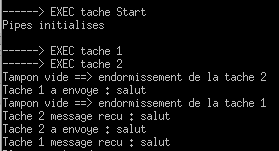
\includegraphics[width=0.8\textwidth]{screens/pipe.PNG}
		\caption{Résultat du pipe}
		\label{pipe}
\end{figure}

On constate que notre système de tubes fonctionne bien. La tâche B reçoit bien le message de A et est capable de lui renvoyer. La tâche A reçoit bien le retour de B.


\end{document}

